% Chapter 1

\chapter{Hardware Results} % Write in your own chapter title
\label{Chapter6}
\lhead{Chapter 6. \emph{Hardware Results}} % Write in your own chapter title to set the page header
\section{Output Voltage}
The output of Hardware circuit is shown below, the frequency can be verified that is 50Hz.
\begin{figure}[htbp]
	\centering
	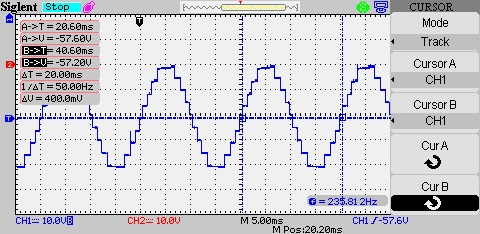
\includegraphics[width = 6in]{./Figures/Photos/Hardware/2}
	\rule{35em}{1pt}
	\caption{Output Voltage at 50Hz}
\end{figure}

The 9 levels in output waveform can be verified. The Value of voltage applied to H-Bridge 1 is 10V and the voltage applied to H-Bridge 2 is 30V i.e 3 times 10. The Switching sequence applied to all switches is shown in previous chapter. The maximum voltage is 40V and minimum voltage is -40V making it sinusoidal. The complete load parameters are shown in below figure.

\begin{figure}[htbp]
	\centering
	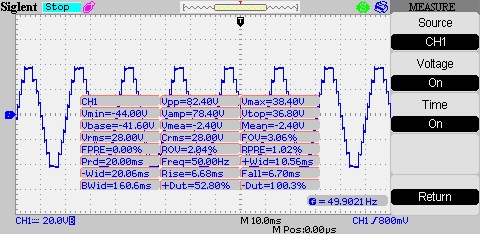
\includegraphics[width = 6in]{./Figures/Photos/Hardware/15}
	\rule{35em}{1pt}
	\caption{Output Voltage with all Load Parameters}
\end{figure}
\newpage
\section{Verification of Conduction Angles}
The conduction angles that we need to verified are given in the below table:
\begin{center}
	\begin{tabular}{ |p{4cm}||p{4cm}|  }
		\hline
		\multicolumn{2}{|c|}{Conduction Angles} \\
		\hline
		Angle & Value in Degrees\\
		\hline
		$\alpha1$ & 6$^o$\\
		\hline
		$\alpha2$ & 22$^o$\\
		\hline
		$\alpha3$ & 38$^o$\\
		\hline
		$\alpha4$ & 60$^o$\\
		\hline
	\end{tabular}
\end{center}
\subsection{Verification of $\alpha1$ }
To verify $\alpha1$ we need to calculate the time delay first step and divide it to total time period and than multiply it with 360.
From the figure shown below:

\begin{equation}
\Delta T = 0.3ms
\end{equation}
\begin{equation}
T = 20ms
\end{equation}
\begin{equation}
\alpha1 = 360*\frac{\Delta T}{T}
\end{equation}
\begin{equation}
\alpha1 = 360*\frac{0.3ms}{20ms}
\end{equation}
\begin{equation}
\alpha1 = 5.4^o
\end{equation}

\begin{figure}[htbp]
	\centering
	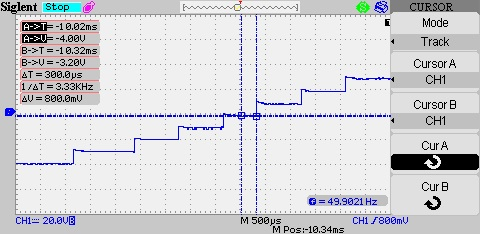
\includegraphics[width = 6in]{./Figures/Photos/Hardware/18}
	\rule{35em}{1pt}
	\caption{Verification of $\alpha1 = 6^o$}
\end{figure}
\newpage
\subsection{Verification of $\alpha2$ }
To verify $\alpha2$ we need to calculate the time delay of second step and divide it to total time period and than multiply it with 360.
From the figure shown below:

\begin{equation}
\Delta T = 1.22ms
\end{equation}

\begin{equation}
T = 20ms
\end{equation}

\begin{equation}
\alpha1 = 360*\frac{\Delta T}{T}
\end{equation}

\begin{equation}
\alpha1 = 360*\frac{1.22ms}{20ms}
\end{equation}

\begin{equation}
\alpha1 = 21.96^o
\end{equation}

\begin{figure}[htbp]
	\centering
	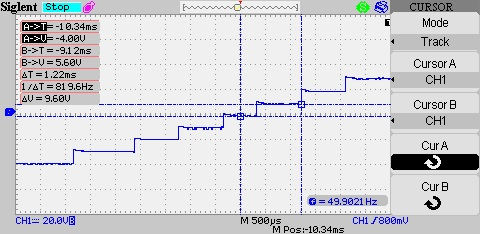
\includegraphics[width = 6in]{./Figures/Photos/Hardware/22}
	\rule{35em}{1pt}
	\caption{Verification of $\alpha2 = 22^o$}
\end{figure}

\newpage
\subsection{Verification of $\alpha3$ }
To verify $\alpha3$ we need to calculate the time delay of third step and divide it to total time period and than multiply it with 360.
From the figure shown below:

\begin{equation}
\Delta T = 2.10ms
\end{equation}

\begin{equation}
T = 20ms
\end{equation}

\begin{equation}
\alpha1 = 360*\frac{\Delta T}{T}
\end{equation}

\begin{equation}
\alpha1 = 360*\frac{2.10ms}{20ms}
\end{equation}

\begin{equation}
\alpha1 = 37.8^o
\end{equation}

\begin{figure}[htbp]
	\centering
	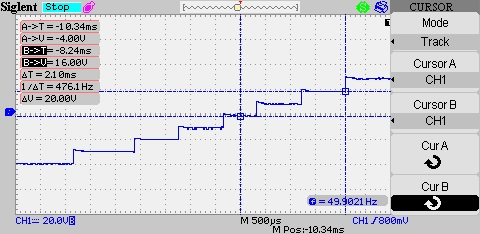
\includegraphics[width = 6in]{./Figures/Photos/Hardware/23}
	\rule{35em}{1pt}
	\caption{Verification of $\alpha3 = 38^o$}
\end{figure}

\newpage
\subsection{Verification of $\alpha4$ }
To verify $\alpha3$ we need to calculate the time delay of fourth step and divide it to total time period and than multiply it with 360.
From the figure shown below:

\begin{equation}
\Delta T = (2.10 + 1.2)ms
\end{equation}

\begin{equation}
T = 20ms
\end{equation}

\begin{equation}
\alpha1 = 360*\frac{\Delta T}{T}
\end{equation}

\begin{equation}
\alpha1 = 360*\frac{(2.10 + 1.2)ms}{20ms}
\end{equation}

\begin{equation}
\alpha1 = 59.4^o
\end{equation}

\begin{figure}[htbp]
	\centering
	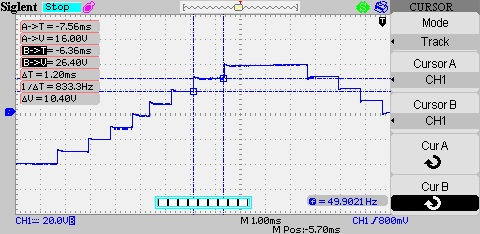
\includegraphics[width = 6in]{./Figures/Photos/Hardware/26}
	\rule{35em}{1pt}
	\caption{Verification of $\alpha4 = 60^o$}
\end{figure}
\newpage
\section{AND Operation with 10KHz PWM}
Below is the results of AND Operation with 10KHz PWM.
\begin{figure}[htbp]
	\centering
	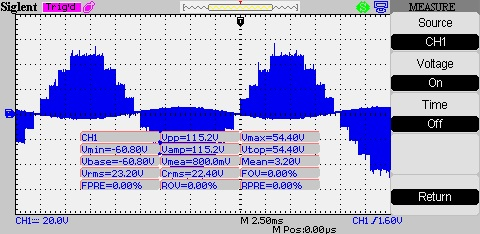
\includegraphics[width = 6in]{./Figures/Photos/Hardware/32}
	\rule{35em}{1pt}
	\caption{AND Operation with 10KHz PWM}
\end{figure}
\newpage
\section{PWM Operation}
Below is the results when PWM Operation at 10KHz is applied.
\begin{figure}[htbp]
	\centering
	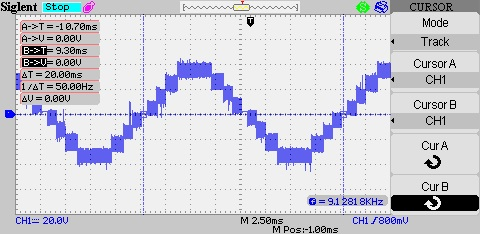
\includegraphics[width = 6in]{./Figures/Photos/Hardware/51}
	\rule{35em}{1pt}
	\caption{PWM Operation at 10KHz}
\end{figure}

\section{Frequency Control}
The frequency can be easily change by programming. Below is the result when the output frequency is 200Hz.
\begin{figure}[htbp]
	\centering
	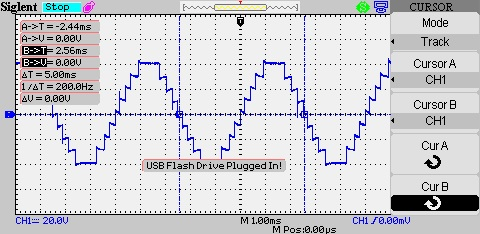
\includegraphics[width = 6in]{./Figures/Photos/Hardware/31}
	\rule{35em}{1pt}
	\caption{Frequency = 200Hz}
\end{figure}

\section{Voltage Control}
The output voltage can be controlled by taking AND Operation with a PWM signal at 10KHz frequency. Now by changing the value of duty cycle we can change the output voltage. Below are the figures showing output voltage at different duty cycles.
\newline
\newline
\textbf{Duty Cycle = 100\%}
\begin{figure}[htbp]
	\centering
	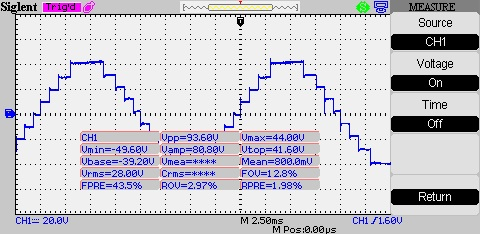
\includegraphics[width = 6in]{./Figures/Photos/Hardware/33}
	\rule{35em}{1pt}
	\caption{Duty Cycle = 100\%}
\end{figure}

\textbf{Duty Cycle = 90\%}
\begin{figure}[htbp]
	\centering
	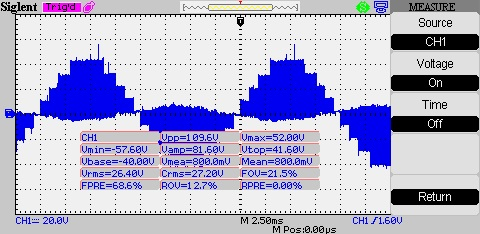
\includegraphics[width = 6in]{./Figures/Photos/Hardware/34}
	\rule{35em}{1pt}
	\caption{Duty Cycle = 90\%}
\end{figure}


\textbf{Duty Cycle = 80\%}
\begin{figure}[htbp]
	\centering
	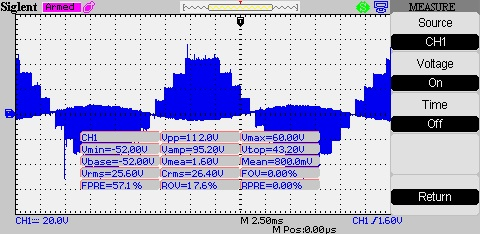
\includegraphics[width = 6in]{./Figures/Photos/Hardware/35}
	\rule{35em}{1pt}
	\caption{Duty Cycle = 80\%}
\end{figure}


\textbf{Duty Cycle = 70\%}
\begin{figure}[htbp]
	\centering
	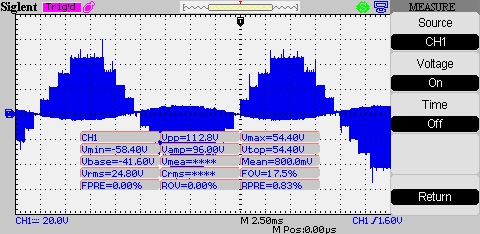
\includegraphics[width = 6in]{./Figures/Photos/Hardware/36}
	\rule{35em}{1pt}
	\caption{Duty Cycle = 70\%}
\end{figure}


\textbf{Duty Cycle = 60\%}
\begin{figure}[htbp]
	\centering
	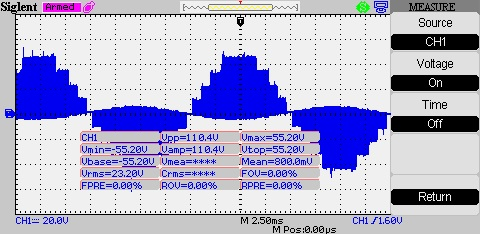
\includegraphics[width = 6in]{./Figures/Photos/Hardware/37}
	\rule{35em}{1pt}
	\caption{Duty Cycle = 60\%}
\end{figure}

\newpage
\textbf{Duty Cycle = 50\%}
\begin{figure}[htbp]
	\centering
	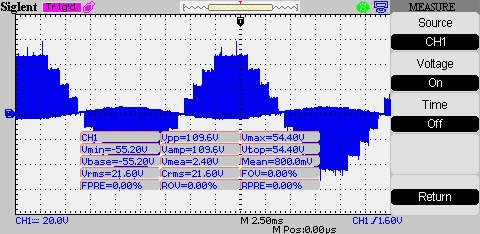
\includegraphics[width = 6in]{./Figures/Photos/Hardware/38}
	\rule{35em}{1pt}
	\caption{Duty Cycle = 50\%}
\end{figure}

\newpage
\textbf{Duty Cycle = 40\%}
\begin{figure}[htbp]
	\centering
	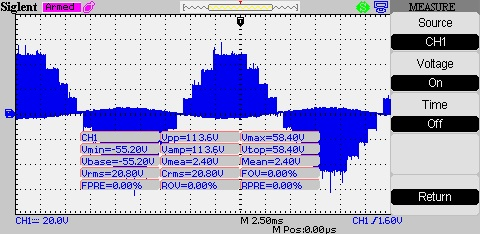
\includegraphics[width = 6in]{./Figures/Photos/Hardware/39}
	\rule{35em}{1pt}
	\caption{Duty Cycle = 40\%}
\end{figure}


\textbf{Duty Cycle = 30\%}
\begin{figure}[htbp]
	\centering
	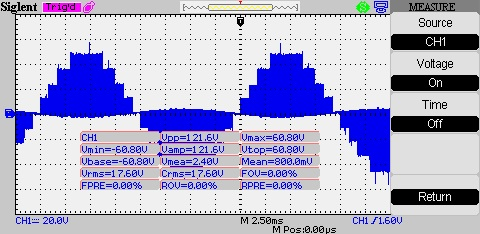
\includegraphics[width = 6in]{./Figures/Photos/Hardware/40}
	\rule{35em}{1pt}
	\caption{Duty Cycle = 30\%}
\end{figure}

\newpage
\textbf{Duty Cycle = 20\%}
\begin{figure}[htbp]
	\centering
	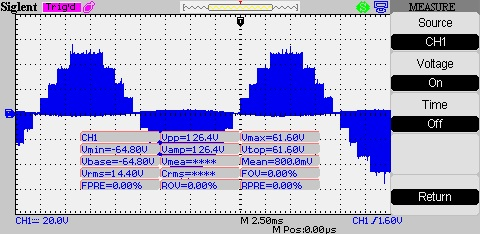
\includegraphics[width = 6in]{./Figures/Photos/Hardware/41}
	\rule{35em}{1pt}
	\caption{Duty Cycle = 20\%}
\end{figure}


\textbf{Duty Cycle = 10\%}
\begin{figure}[htbp]
	\centering
	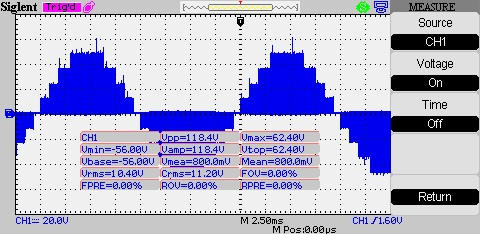
\includegraphics[width = 6in]{./Figures/Photos/Hardware/42}
	\rule{35em}{1pt}
	\caption{Duty Cycle = 10\%}
\end{figure}

\newpage
\textbf{Duty Cycle = 5\%}
\begin{figure}[htbp]
	\centering
	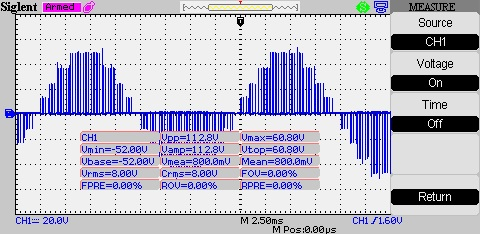
\includegraphics[width = 6in]{./Figures/Photos/Hardware/43}
	\rule{35em}{1pt}
	\caption{Duty Cycle = 5\%}
\end{figure}

\textbf{Duty Cycle = 2\%}
\begin{figure}[htbp]
	\centering
	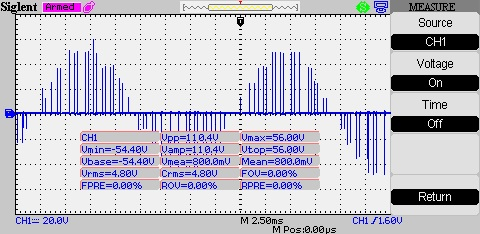
\includegraphics[width = 6in]{./Figures/Photos/Hardware/44}
	\rule{35em}{1pt}
	\caption{Duty Cycle = 2\%}
\end{figure}
\newpage
\textbf{Duty Cycle = 1\%}
\begin{figure}[htbp]
	\centering
	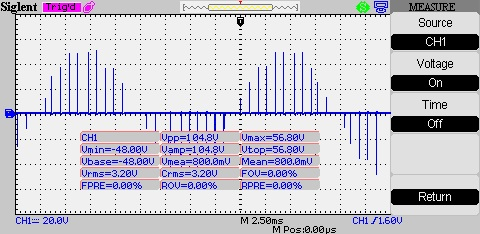
\includegraphics[width = 6in]{./Figures/Photos/Hardware/45}
	\rule{35em}{1pt}
	\caption{Duty Cycle = 1\%}
\end{figure}

\textbf{Duty Cycle = 0\%}
\begin{figure}[htbp]
	\centering
	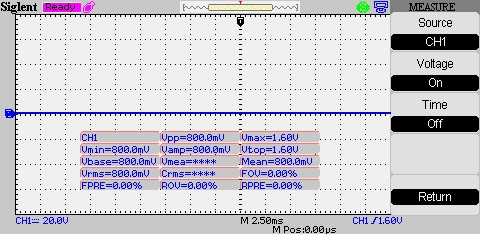
\includegraphics[width = 6in]{./Figures/Photos/Hardware/46}
	\rule{35em}{1pt}
	\caption{Duty Cycle = 0\%}
\end{figure}
\subsection{Table }
\begin{center}
	\begin{tabular}{ |p{4cm}||p{4cm}|  }
		\hline
		\multicolumn{2}{|c|}{Vriaion of $V_output$(RMS) w.r.t Duty cycle} \\
		\hline
		Duty Cycle (\%) & $V_{output}$(RMS)\\
		\hline
		100 & 28 \\
		\hline
        90 & 26.4\\
        \hline
        80 & 25.6 \\
        \hline
        70 & 24.8 \\
        \hline
        60 & 23.20 \\
        \hline
        50 & 21.6 \\
        \hline
        40 & 20.8 \\
        \hline
        30 & 17.6 \\
        \hline	
        20 & 14.4 \\
        \hline	
        10 & 10.4 \\
        \hline
        5 & 8 \\
        \hline
        2 & 4.8 \\
        \hline
        1 & 3.2 \\
        \hline
        0 & 0.8 \\
        \hline
	\end{tabular}
\end{center}

\subsection{Relation Between Duty Cycle and V$_{rms}$}
\begin{figure}[htbp]
	\centering
	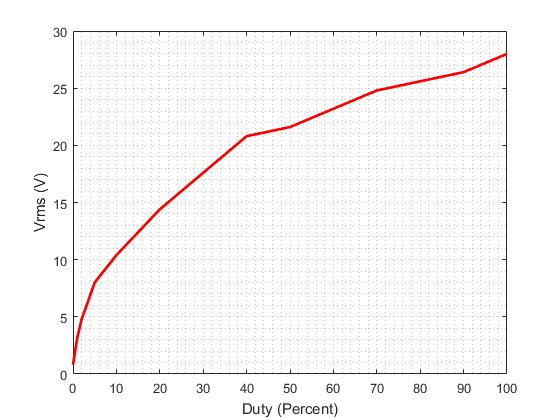
\includegraphics[width = 5in]{./Figures/p_d_v}
	\rule{35em}{1pt}
	\caption{Relation Between Duty Cycle and V$_{rms}$}
\end{figure}

\section{Voltage and Current Parameters}
Below is the load parameters when 100W load is connected at the output terminals.
\begin{equation}
V_{H-Bridge-1} = 50V
\end{equation} 
\begin{equation}
V_{H-Bridge-2} = 150V
\end{equation} 
\begin{equation}
Vout_{rms} = 150V
\end{equation} 
\begin{equation}
Iout_{rms} = 2.205A
\end{equation} 
\begin{center}
	\begin{tabular}{ |p{4cm}||p{4cm}|p{4cm}|  }
		\hline
		\multicolumn{3}{|c|}{Load Parameters} \\
		\hline
		Component & Voltage & Current \\
		\hline
		Isolated Supplies for Gate Driver & 15V & 14mA\\
				\hline
		TLP250 Input (Gate Driver) & 3.3V & 15mA\\
				\hline
		TLP250 Output (Gate Driver) & 15V & 14mA\\
				\hline
		IRF450 (H-Bridge-1) & 50V$_{rms}$ & 0.7352A\\
				\hline
		IRF450 (H-Bridge-2) & 150V$_{rms}$ & 2.205A\\
				\hline
		STM32F4 (GPIO Pins) & 3.3V & 15mA\\
		\hline
	\end{tabular}
\end{center}
